\documentclass[10pt,preprint]{sigplanconf}
\usepackage[utf8]{inputenc}
\usepackage{graphicx}
\usepackage{fancyhdr}
\usepackage{amsmath}
\usepackage{xfrac}
\usepackage{listings}
\usepackage{tikz}
\usetikzlibrary{trees,automata,positioning,arrows}
\usepackage[sc]{mathpazo}
\usepackage{titlesec}
\usepackage{etoolbox}
\usepackage{mathtools}
\usepackage{bussproofs}
\usepackage[numbers]{natbib}
\DeclarePairedDelimiter{\ceil}{\lceil}{\rceil}

\newcommand{\mytitle}{Timing-sensitive Secure Multi-Execution}
\authorinfo{Christopher Schuster}
           {University of California, Santa Cruz}
           {\texttt{\{cschuste\}@ucsc.edu}}


\title{\mytitle}
% \pagestyle{fancy}
% \fancyhf{}
% \titleformat{\section}{\normalfont\Large\bfseries}{}{0em}{}
% \titleformat{\subsection}{\normalfont\bfseries}{}{0em}{}
% \renewcommand{\thesection}{\arabic{section}}
% \renewcommand{\thesubsection}{\arabic{section}.\alph{subsection})}
\tikzstyle{t} = [circle, draw=black, thick, fill=none, text centered, minimum height=8mm,minimum width=8mm]
\tikzstyle{level 1}=[level distance=1.5cm, sibling distance=2cm]
\tikzstyle{level 2}=[level distance=1.5cm, sibling distance=1cm]
\tikzstyle{level 3}=[level distance=1.5cm, sibling distance=1cm]
\tikzstyle{level 4}=[level distance=1.5cm, sibling distance=1cm]
% \lhead{\myauthor}
% \rhead{\mytitle}
% \cfoot{\thepage}
% \newcommand{\zerodisplayskips}{%
%   \setlength{\abovedisplayskip}{0pt}
%   \setlength{\belowdisplayskip}{0pt}
%   \setlength{\abovedisplayshortskip}{0pt}
%   \setlength{\belowdisplayshortskip}{0pt}}
% \appto{\normalsize}{\zerodisplayskips}
% \appto{\small}{\zerodisplayskips}
% \appto{\footnotesize}{\zerodisplayskips}
\lstdefinelanguage{JavaScript}{
  keywords={typeof, new, true, false, catch, function, return, null, catch, switch, var, if, in, while, do, else, case, break, fx},
  keywordstyle=\color{darkgray}\bfseries,
  ndkeywords={class, export, boolean, throw, implements, import, this},
  ndkeywordstyle=\color{darkgray}\bfseries,
  identifierstyle=\color{black},
  sensitive=false,
  comment=[l]{//},
  morecomment=[s]{/*}{*/},
  commentstyle=\color{purple}\ttfamily,
  stringstyle=\color{gray}\ttfamily,
  morestring=[b]',
  morestring=[b]"
}

\lstset{language=JavaScript,
        basicstyle=\ttfamily,
        aboveskip={0.5\baselineskip},
        belowskip={0.5\baselineskip},
        showstringspaces=false,
        frame=tb,
        captionpos=b}
% Don't indent paragraphs.
% \setlength{\parindent}{0em}
% \setlength{\parskip}{0.5\baselineskip}
% \newcommand{\prob}[1]{\setcounter{section}{#1} \addtocounter{section}{-1} \section{} }
\newcommand{\lab}[1]{\RightLabel{\textsc{\small #1}}}
\newcommand{\ov}[2]{\genfrac{}{}{0pt}{}{\text{\textbf{#1}}}{\text{\footnotesize{#2}}}}
\renewcommand{\t}[1]{~\text{#1}~}
\newenvironment{bpt}{\leavevmode\hbox\bgroup}{\DisplayProof\egroup}
\begin{document}
\maketitle

\abstract{Bla bla}

\section{Introduction}

Secure information flow ensures that private information can never leak to or indirectly influence public/un-authorized recipients.  However, if the program performs both private and non-private computation on the same machine, an external observer might learn about non-private data simply through the timing covert channel.

As an example, the following NodeJS JavaScript web server has an internal ``private'' request counter which gets incremented at every request and logged to a local console.

\subsection{Secure multi execution}

Secure multi-execution as introduced by Devriese et al. \cite{devriese2010} protects against both direct and indirect information leaks by executing the program more than once.  Each execution has a security level, e.g. H and L, and can only read and write information on that same level.  Reading from a lower level will use a cached values from a previous read, reading from a higher level returns a default value; writing to a lower or higher level will be ignored.

For the example in Listing \ref{lst:express}, secure multi execution could ensure that the private information in the \verb+counter+ variable cannot influence public observable output.  The \emph{public} thread of execution reads a default value for the counter, e.g. 0, and suppresses the update and the \verb+console.log+ call while the \emph{private} thread of execution skips the \emph{res.send} call.

\begin{lstlisting}[float,label=lst:express,caption={JavaScript Server Code which leaks the value of the private request counter via the timing covert channel.}]
var app = require('express')();
var counter = 0;   // Private counter

app.post('/', function (req, res) {
  counter++;
  for (var i = 0; i < counter; i++) {
    console.log('.');
  }
  res.send('Request counted.');
});

var server = app.listen(3000);
\end{lstlisting}

\subsection{Timing covert channels}

Despite information flow control through secure multi execution, the code shown in Listing \ref{lst:express} is still vulnerable to attacks through the timing covert channel.  If the \verb+console.log+ function takes a certain time, an attacker sending HTTP requests might measure the time between request and response which will depend on the secret value of the counter.

In order to close this timing covert channel, the private and public execution threads need to be disentangled and scheduled in a way that prevents an attacker from learning about other concurrently executing threads.

Kashyap et. al.~\cite{kashyap2011} previously explored different scheduling strategies for termination and timing-sensitive secure multi execution.  The simplest possible scheduling strategies always prioritizes public execution over private execution and thereby hides concurrent private execution, which may depend on private data, from public execution with its externally observable timing.  However, this might cause private execution threats to starve and it does not work if there are more security levels than just private and public.

\begin{figure}
\begin{center}\vspace{-2ex}
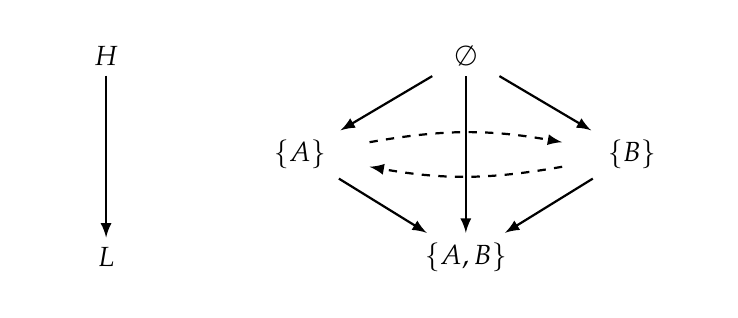
\begin{tikzpicture}
\tikzstyle{c} = [minimum width=5em]
\tikzstyle{d} = [rectangle, draw, thick, minimum height=6.5mm,minimum width=5em]
\matrix[column sep=1em,row sep=2em]
{
  \node[c] (h) {$H$}; & & & \node[c] (ab) {$\emptyset$}; & \\
                      & & \node[c] (a) {$\{A\}$}; & & \node[c] (b) {$\{B\}$}; \\
  \node[c] (l) {$L$}; & & & \node[c] (n) {$\{A,B\}$}; & \\
};
\draw[-latex, thick] (h) -- (l);
\draw[-latex, thick] (ab) -- (a);
\draw[-latex, thick] (ab) -- (b);
\draw[-latex, thick] (a) -- (n);
\draw[-latex, thick] (b) -- (n);
\draw[-latex, thick] (ab) -- (n);
\draw[-latex, thick, dashed] (a) to [bend left=10] (b);
\draw[-latex, thick, dashed] (b) to [bend left=10] (a);
\end{tikzpicture}
\end{center}
\caption{In contrast to the simple binary $HL$ security lattice, more complex security lattices only have a partial order.  Here, $\{ A,B \}$, the public security level of information that both $A$ and $B$ can access, might influence other security levels but should not be influenced by information private to either $A$ or $B$.  The two security levels $A$ and $B$, on the other hand, are incomparable.}
\label{fig:lattice}
\end{figure}

Figure \ref{fig:lattice} shows two different designs of possible security levels, the simple public/private binary system, and a more complex lattice with additional two principals $A$ and $B$ who can designate information as private for each individually.  In contrast to the simple $H/L$ lattice, execution that is private for $A$ and execution that is private for $B$ have to be hidden from each other.  This means that both execution threads are incomparable in terms of scheduling priority.  Furthermore, the maximum execution time available to each security level cannot be influenced by timing and termination of other incomparable security levels.

\section{Formalism}

Consider a programming language based on lambda calculus with IO channels as shown in Figure \ref{fig:lang}.  Each channel is opened with a fixed security label $l$ and a language-specific name $n$, e.g. the path to a file, and allows blocking reads and writes.

Evaluating this language uses a mapping $\Gamma$ from channel $ch$ to a sequence $\vec{n}$ of primitive values, e.g. byte or strings.  A single thread of execution can be either ready $R$, blocked on a channel $B/ch$ or terminated $T$.  While $\rightarrow$ denotes a step of evaluation of a single thread, $\Rightarrow$ is a transition of a system of threads, one for each security label $l$ with specific scheduling.  The complete operational semantics are shown in Figure \ref{fig:lang}.

\begin{figure*}
\[ \arraycolsep=1.6pt\def\arraystretch{1.5}
\begin{array}{rl}
  \multicolumn{2}{l}{x : \t{Identifier} \hfill n : \t{Literal} \hfill ch : \t{Channel} \hfill l : \t{Security label}} \\
  \multicolumn{2}{l}{
    S = \{ R, B/ch, T \} \hfill
    \Gamma : ch \mapsto \vec{n} \hfill
    p : \Gamma \times S \times L \times e} \\[1em]
  e := & n ~|~ \lambda x.~e ~|~ x ~|~ e ~ e ~|~ e ; e ~| \t{open} l~e ~| \t{read} e ~| \t{write} e~e ~|~ch\\
    v := & n ~|~ \lambda x.~e ~|~ ch \\[1em]
  E[\circ] := & \circ ~|~E~e~|~v~E~| \t{open} l~E~| \t{read} E~| \t{write} E~e~| \t{write} v~E~|~E~;~e
  \end{array} \\[1em]
\]
\begin{center}
\begin{bpt}
  \AxiomC{$\Gamma, L, e \rightarrow \Gamma', S, e' $}
  \lab{e-ctx}
  \UnaryInfC{$\Gamma, L, E[e] \rightarrow \Gamma', S, E[e'] $}
\end{bpt} \hspace{1em}
\begin{bpt}
  \AxiomC{}
  \lab{e-app}
  \UnaryInfC{$\Gamma, L, (\lambda x. e)~v \rightarrow \Gamma, R, e[x \mapsto v] $}
\end{bpt} \hspace{1em}
\begin{bpt}
  \AxiomC{}
  \lab{e-seq}
  \UnaryInfC{$\Gamma, L, (v~;~e) \rightarrow \Gamma, R, e $}
\end{bpt} \\[2em]
\begin{bpt}
  \AxiomC{$ch~\t{fresh} ~~~ \Gamma' = \Gamma[ch \mapsto ()]$}
  \lab{e-open}
  \UnaryInfC{$\Gamma, L, \t{open} l~n \rightarrow \Gamma', R, ch $}
\end{bpt} \hspace{1em}
\begin{bpt}
  \AxiomC{$\Gamma(ch) ...  $}
  \lab{e-write}
  \UnaryInfC{$\Gamma, L, \t{write} ch~n \rightarrow \Gamma, R, e $}
\end{bpt} \\[2em]
\begin{bpt}
  \AxiomC{}
  \lab{e-read}
  \UnaryInfC{$\Gamma, L, \t{read} ch \rightarrow \Gamma', R, v $}
\end{bpt} \hspace{1em}
\begin{bpt}
  \AxiomC{}
  \lab{e-read-block}
  \UnaryInfC{$\Gamma, L, \t{read} ch \rightarrow \Gamma, B/ch, \t{read} ch $}
\end{bpt}
\end{center}
\caption{Operational semantics of the language shown in Figure \ref{fig:lang}.}
\label{fig:lang}
\end{figure*}

\section{Scheduling}

Scheduling to prevent time-sensitive non-interference *and* starvation between comparable and non-comparable threads.

Scheduling vector $v$ with slots $i=1 \ldots \infty$.  Scheduling probability $p(i) = 2^{-i}$ with $\sum_i p(i) = 1$.

When thread $t$ changes from Ready to Blocked,

\begin{itemize}
  \item swap schedule position of $t$ with thread $t'$ with $l_{t'} \sqsubseteq l_t$ and $t'$ is the last such thread.
\end{itemize}

When thread $t$ changes from Blocked to Ready or gets created.

\begin{itemize}
  \item if newly created, add $t$ add the end of $v$;
  \item swap schedule position of $t$ with thread $t'$ with $l_{t} \sqsubseteq l_{t'}$ and $t'$ is the first such thread.
\end{itemize}

When thread $t$ terminates.

\begin{itemize}
  \item if $t$ was last non-terminated thread at this level in the lattice, just remove it from $v$;
  \item otherwise, assign $t'$ to the slot of $t$ with $l_{t'} \sqsubseteq l_t$ and $t'$ is the last such thread.
\end{itemize}

Randomized scheduling:

\begin{enumerate}
  \item Initialize $i$ with 1.
  \item If $v_i$ is not runnable, remain idle.
  \item With $p(i)$ probability, schedule $v_i$.
  \item Otherwise, increment $i$ and repeat from step 2.
\end{enumerate}

Round-robin scheduling:

\begin{enumerate}
  \item Initialize $i$ with 1.
  \item If $v_i$ is not runnable, remain idle.
  \item If $i$ was skipped at the last scheduling decision for $i$, schedule $v_i$.
  \item Otherwise, skip it, increment $i$ and repeat from step 2.
\end{enumerate}

\subsection{Timing attacks}



\section{Related work}

It is actually possible to ensure timing-sensitive non-interference while still allowing branches on private values, as shown by Kashyap et. al.~\cite{kashyap2011}.  They recognized that a custom scheduler could schedule public/low threads in a way that these cannot learn anything about the potential execution of higher/private threads.  Different scheduling strategies correspond to different trade-offs between correctness/starvation and performance.  Non-comparable labels in a lattice ($l \not \sqsubseteq l'~\wedge~l \not \sqsupseteq l'$) further complicate scheduling as two non-comparable threads have to be hidden from each other.  Nevertheless, timing-sensitive non-interference is actually possible and subsumes termination-sensitive non-interference.

\section{Evaluation}



\section{Conclusions}


\bibliographystyle{unsrtnat}
\bibliography{references}

\end{document}
